\documentclass[10pt]{article}
\usepackage[margin=0.58in]{geometry}
\usepackage{booktabs,enumitem,fancyhdr,graphicx,tabularx,titlesec}
\usepackage[hidelinks]{hyperref}
\graphicspath{{docs/lessons/assets/}{../assets/}}
\hypersetup{pdftitle={ADK Lesson 054: Inert Infrared Command Translator},
 pdfauthor={Kevin Shanahan},
 pdfsubject={Fixed semantic translation, atomic coordination, self-echo suppression, and attributed round-trip replay},
 pdflang={en-US}}
\pagestyle{fancy}\fancyhf{}
\lhead{\textsc{ADK Lesson 054}}\rhead{Inert IR Command Translator}
\cfoot{\thepage}\setlength{\headheight}{14pt}
\setlength{\parindent}{0pt}\setlength{\parskip}{2.5pt}
\setlist{nosep,leftmargin=1.45em}
\titleformat{\section}{\Large\bfseries}{\thesection}{0.5em}{}
\newcommand{\lessonbox}[1]{\begin{center}\fbox{\parbox{0.92\linewidth}{#1}}\end{center}}
\newcommand{\blankline}{\rule{0.72in}{0.4pt}}

\begin{document}
\small
\begin{center}
 {\Huge\bfseries Inert IR Command Translator}\\[3pt]
 {\Large Map one valid copied symbol to a different local symbol}\\[7pt]
 \fbox{\textbf{E0 POLICY COMPOSITION --- NO RECEIVER, EMITTER, OR DEVICE CONTROL}}
\end{center}
\begin{tabularx}{\linewidth}{@{}>{\bfseries}l X >{\bfseries}l X@{}}
Lesson & 054 --- project & Time & 150--210 minutes\\
Prerequisites & Lessons 052 and 053 & Board & compile-only Mega replay\\
Evidence & distinct named memory cells & Boundary & fixed allowlist only\\
\end{tabularx}

\lessonbox{\textbf{Project boundary.} \texttt{InertIrTranslator} composes
copied receive evidence with an immutable local emission catalog. It owns no
receiver, emitter, pin, timer, interrupt, carrier endpoint, display, bus,
supply, or optical path. It is not a learning remote, replay bridge, or
unknown-protocol transmitter.}

\section{Translate through a fixed different-symbol map}
\begin{tabularx}{\linewidth}{@{}l l X@{}}
\toprule
Valid received symbol & Local output symbol & Rule\\
\midrule
\texttt{StationPing} & \texttt{StationReady} & fixed firmware mapping\\
\texttt{StationReady} & \texttt{StationAcknowledge} & fixed firmware mapping\\
\texttt{StationCancel} & none & cancellation dominates\\
\texttt{StationAcknowledge} & \texttt{StationPing} & fixed firmware mapping\\
\bottomrule
\end{tabularx}

Only \texttt{KnownValid}, \texttt{IntegrityVerified} evidence from the
configured qualified source can select a mapping. Every output differs from
its input. Repeat, unknown, malformed, truncated, overflowed, stale,
source-faulted, self-echo, and unlisted records remain visible but cannot
become transmit authority.

\begin{center}
% ADK visual: pencil
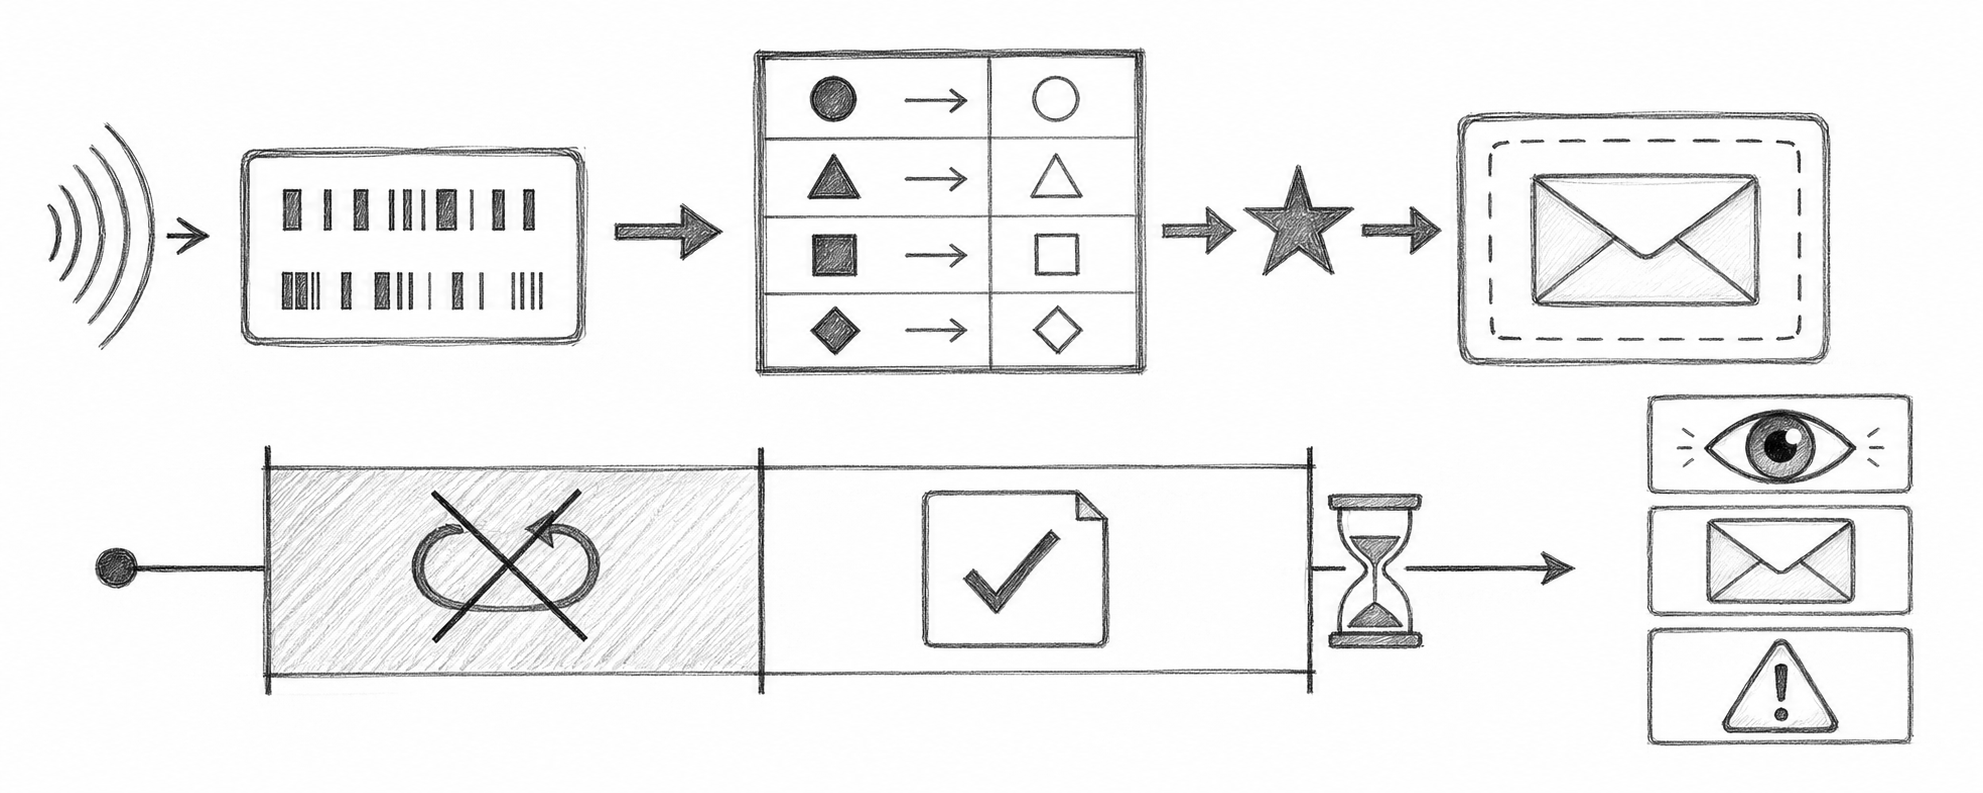
\includegraphics[width=0.98\linewidth,height=0.31\textheight,
 keepaspectratio]{054-translator-window-pencil.png}

\small\textit{Alternative text: graphite copied marks enter a fixed
different-symbol table and then a bounded envelope card. Below, a crossed
self-echo interval precedes a checked response window and hourglass boundary;
eye, envelope, and warning result cells remain separate.}
\end{center}

\section{Admit one complete atomic envelope}
\texttt{IrTranslatorUpdateInput} carries cancellation, a prepared commit,
receive evidence, and actual-emission evidence at one supplied time. Validate
the complete envelope before mutation, then apply fixed precedence:

\begin{enumerate}
 \item reject a structurally invalid envelope without mutation;
 \item preserve an already latched dependency or safety fault;
 \item apply matching cancellation and invalidate both candidates;
 \item copy and classify receive evidence;
 \item correlate actual-emission evidence;
 \item commit a still-current parent and child candidate; and
 \item publish presentation intent last.
\end{enumerate}

There are no separate receive, cancel, commit, or emission entry points whose
caller-selected order could change the result.

\section{Bind parent and child capabilities}
\texttt{prepareTranslation(operationId, now)} uses only the current Lesson
052 evidence generation and fixed map. Its preview binds translator owner,
epoch, configuration, mapping digest, parent generation, operation, copied
input digest, receive provenance, evidence generation, different output
symbol, catalog identity, and the complete Lesson 053 child preview.

A foreign, stale, reconstructed, reused, reset-invalidated, or
shutdown-invalidated preview rejects. A simultaneous valid cancellation
invalidates parent and child before either commits. After complete preflight,
the child commit and parent publication describe one attributable semantic
operation, not optical emission.

\section{Separate logical intent from actual emission evidence}
A policy commit is not optical start. Round-trip correlation begins only when
qualified \texttt{IrEmitterEvidence} supplies the exact source, transaction,
actual start, actual completion, and status. E0 supplies explicitly synthetic
values.

\begin{center}
\begin{tabularx}{0.92\linewidth}{@{}l X@{}}
\toprule
Half-open interval & Classification\\
\midrule
\([\textit{actual start},\textit{actual completion}+\textit{guard})\) &
\texttt{SelfEchoSuppressed}; visible, never a response\\
\([\textit{response start},\textit{response start}+\textit{window})\) &
eligible only after every attribution check\\
exact response end & timeout; exclusive boundary\\
\bottomrule
\end{tabularx}
\end{center}

All interval arithmetic uses unsigned modular half-range comparison. Overflow,
regression, and exact-half-range ambiguity reject or fault atomically.
Lesson 052 supplies observation time, not optical arrival time, so E0 proves
only deterministic observation-time correlation.

\newpage
\section{Publish one complete round-trip record}
A successful \texttt{IrRoundTripResult} atomically binds operation and output
symbol, catalog identity, transmitter source, actual start and completion,
elapsed duration, receive disposition and strength, complete receive
provenance and generation, and correlation status.

Payload equality alone is insufficient. Source, mapping, catalog, operation,
transaction, emission evidence, expected response symbol, self-echo exclusion,
and response window must all agree. Fields from different updates cannot be
assembled into a success.

\section{Keep result cells independent}
\begin{tabularx}{\linewidth}{@{}l X X@{}}
\toprule
Cell & Shows & Never grants\\
\midrule
receive & identity, disposition, strength & transmission authority\\
translation & fixed different-symbol candidate & electrical emission\\
transmit & envelope intent and attribution & optical success\\
self-echo & bounded suppressed count & valid response\\
round trip & complete correlated record & hardware qualification\\
fault & independent presentation intent & authority or cancellation\\
\bottomrule
\end{tabularx}

These memory cells are the E0 non-Serial observation path. Compilation does
not prove that a powered Mega executed the sketch.

\section{Run the deterministic project workbook}
\begin{enumerate}
 \item Initialize both children and the translator. Predict inactive intent,
       empty round trip, and distinct receive, transmit, and fault cells.
 \item Admit each valid mapping and prove every output differs from its input.
 \item Try repeat, unknown, malformed, stale, unlisted, and wrong-source
       evidence. Verify visibility without a translation candidate.
 \item Prepare a translation, then try foreign, stale, changed, consumed,
       reset-invalidated, and shutdown-invalidated previews.
 \item Collide valid cancellation with commit, receive, emission evidence,
       and presentation failure. Verify cancellation precedence.
 \item Replay actual-emission evidence and receive at one tick before, exactly
       at, and one tick after both the guard and response boundaries.
 \item Exercise rollover, regression, half-range ambiguity, timeout, missed
       service, and suppressed-count saturation.
 \item Replay two instances with identical fixture inputs and compare every
       result field byte-for-byte.
\end{enumerate}

\begin{tabularx}{\linewidth}{@{}X X X X X X@{}}
\toprule
frame & receive & strength & output & envelope & round trip\\
\midrule
\rule{0pt}{16pt}\blankline & \blankline & \blankline & \blankline & \blankline & \blankline\\[8pt]
\blankline & \blankline & \blankline & \blankline & \blankline & \blankline\\[8pt]
\blankline & \blankline & \blankline & \blankline & \blankline & \blankline\\
\bottomrule
\end{tabularx}

\section{Separate acquisition evidence from safe-state evidence}
\textbf{Acquisition prediction and observation.} Valid child configuration,
fixed storage, nonzero epochs, and immutable map/catalog identities allow E0
initialization. Host tests inspect lifecycle, bindings, generations, digests,
and distinct result cells in memory.

\textbf{Acquisition interpretation.} Success proves bounded policy
composition only. It does not prove receiver sampling, carrier generation,
emitted light, a response, or device control.

\textbf{Safe-state prediction and observation.} Construction, cancellation,
completion, fault, shutdown, and restart publish inactive envelope intent and
no pending translation. This is not emergency stop, power removal, or proof
of a dark emitter.

\section{Read the conservative resource evidence}
The final canonical Mega 2560 replay measures 16,162 bytes of flash and 1,343 bytes
of static SRAM. The maximal measured fixture uses 21,864 bytes of flash and
3,531 bytes of static SRAM. \texttt{sizeof(InertIrTranslator)} is 407 bytes,
and its required caller-owned receive storage is another 400 bytes, for 807
bytes at that ownership boundary.

Conservative compiler evidence estimates 888 bytes on the maximal analyzed
stack path. That misses the 800-byte stack target but passes the 1,024-byte
hard limit, leaving about 3,773 bytes after the measured static and stack
allowances on the Mega 2560. These are deliberately conservative compiler and
link-map results for the exact fixtures and toolchain, not runtime high-water
measurements or proof of every interrupt schedule. Any
source, toolchain, optimization, library, interrupt, or aggregate-composition
change requires remeasurement.

\section{Keep powered work outside this lesson}
E1 requires separately qualified exact receiver, emitter and driver, carrier
endpoint, observation path, board, supply, complete resource budgets,
authoritative formal schematic, default-off evidence, and recorded bench
acceptance. Current limiting plus bounded duty reduces exposure but does not
establish eye safety. Unknown devices, access-control commands, high-power or
long-range transmission, and pyrotechnic or launcher control are prohibited.

\end{document}
